% !TEX program = xelatex

\documentclass[a4paper, sans]{article}
\usepackage[T1]{fontenc}
\usepackage[french]{babel}
\usepackage{graphicx}
\usepackage{subfig}
\usepackage{hyperref}
\usepackage{amsmath}
\usepackage{setspace}
\usepackage{placeins}
\usepackage{unnumberedtotoc}
\usepackage{gensymb}
\usepackage{tabularx}

\usepackage[top=30mm, bottom=30mm]{geometry}

\usepackage{listings}

\usepackage[font=small, labelfont=bf]{caption}
\usepackage[nottoc, notlof, notlot]{tocbibind}
\usepackage{fancyhdr}
\pagestyle{fancy}

\hypersetup{
    colorlinks,
    linkcolor={red},
    citecolor={black},
    urlcolor={blue}
}

\date{\today}
\author{Mélanie Legros \\ Nicolas Lépy \\ Simon Perche \\ Hydriss Ruet \\
Université de Technologie de Belfort-Montbéliard}
\title{Projet IN5X - Rapport}

\rhead{\leftmark}
\lhead{}
\lfoot{UTBM}
\rfoot{Mélanie \bsc{Legros}\\Nicolas \bsc{Lépy}\\Simon \bsc{Perche}\\Hydriss \bsc{Ruet}}
\cfoot{\thepage}
\renewcommand{\headrulewidth}{1pt}
\renewcommand{\footrulewidth}{2pt}

\onehalfspacing % Set line spacing to 1.5

\begin{document}
    \begin{titlepage}

      \newcommand{\HRule}{\rule{\linewidth}{0.5mm}} % Defines a new command for the horizontal lines, change thickness here
      
      \centering % Center everything on the page
      
      %----------------------------------------------------------------------------------------
      %	HEADING SECTIONS
      %----------------------------------------------------------------------------------------
      
      \textsc{\LARGE Université de Technologie \\de Belfort-Montbéliard}\\[1.5cm] % Name of your university/college
      \textsc{\Large Informatique}\\[0.5cm] % Major heading such as course name
      \textsc{\large Image, interaction et réalité virtuelle}\\[0.5cm] % Minor heading such as course title
      
      %----------------------------------------------------------------------------------------
      %	TITLE SECTION
      %----------------------------------------------------------------------------------------
      
      \HRule \\[0.4cm]
      { \huge \bfseries Augmented Reality From Scratch\\IN5X - Projet}\\[0.4cm] % Title of your document
      \HRule \\[1.5cm]
      
      %----------------------------------------------------------------------------------------
      %	AUTHOR SECTION
      %----------------------------------------------------------------------------------------

      
      % If you don't want a supervisor, uncomment the two lines below and remove the section above
      \Large \emph{Auteurs :}\\
      Mélanie \bsc{Legros}\\Nicolas \bsc{Lépy}\\Simon \bsc{Perche}\\Hydriss \bsc{Ruet}\\[3cm] % Your name
      
      %----------------------------------------------------------------------------------------
      %	DATE SECTION
      %----------------------------------------------------------------------------------------
      
      {\large \today}\\[2cm] % Date, change the \today to a set date if you want to be precise
      
      %----------------------------------------------------------------------------------------
      %	LOGO SECTION
      %----------------------------------------------------------------------------------------
      
      
\includegraphics[scale=0.18]{img/utbm_logo.png}\\[1cm] % Include a department/university logo - this will require the graphicx package
      
      %----------------------------------------------------------------------------------------
      
      \vfill % Fill the rest of the page with whitespace
      
    \end{titlepage}
    \thispagestyle{empty}

    \clearpage

    \setcounter{tocdepth}{2}
    {\hypersetup{linkcolor=black}
    \tableofcontents }

    \newpage

    %Include tex_files
    \rhead{\bsc{Introduction}}
    \addpart{Introduction}

Le but de ce projet est de construire une application de réalité augmentée "from scratch", c'est-à-dire en essayant de réimplémenter le maximum de méthodes, utilisant le moins possible d'outils déjà existants.

L'application se basera tout de même sur OpenCV, une bibliothèque graphique libre spécialisée dans le traitement d'images.

Plusieurs méthodes sont envisageables pour la création d'une application de réalité augmentée. Certaines méthodes basées sur de la reconstruction de scène 3D avec notamment de la Feature Extraction peuvent être très efficace et ne nécessitent pas de repère dans l'image, mais l'implémentation et les concepts à appréhender sont plus robustes.

Notre application de réalité augmentée se basera sur une méthode basée sur un repère, l'ARTag, qui consiste à placer un marqueur sur l'environnement, permettant à la caméra d'avoir des indications en temps réel sur l'orientation ou la distance des objets virtuels à intégrer à l'environnement selon la forme détectée du marqueur. 

Ce rapport est divisé en trois parties distinctes. Dans un premier temps, nous parlerons de comment détecter l'ARTag sur l'image. Deuxièmement, nous montrerons comment nous avons construit la scène autour de ce tag, à partir de la caméra jusqu'au rendu. Finalement, nous nous pencherons sur les axes d'améliorations de l'application, qui pourraient la rendre plus robuste et réaliste.

% TODO: détailler le from scratch

    \rhead{\leftmark}

    \part{Détection du tag}

La détection du tag est une partie cruciale de cette application de réalité augmentée. L'objectif est de récupérer les coordonnées du tag dans la caméra pour avoir les informations sur l'orientation et la distance de la scène à projeter sur l'image.

    \section{Détection complète}

    La détection du tag consiste à récupérer toutes les formes qui pourraient correspondre au tag dans l'image, puis de trouver la forme qui correspond au véritable tag que nous cherchons. L'orientation et la distance du tag détecté servira ensuite pour projeter les objets dans la scène.

    Une fois le tag détecté, l'application tentera de le tracker lors des images suivantes de la vidéo, afin de gagner en temps de calcul en évitant de refaire tout le processus et de stabiliser le rendu. Si le tracking ne parvient pas à suivre le tag (mouvement trop important de la caméra par exemple), une nouvelle détection complète est effectuée.

        \subsection{Modèle de tag}

        Le tag consiste à une grille en deux dimensions qui représente un code binaire matérialisé par des cases noires ou blanches.

        \begin{figure}[!h]
            \centering
            
\includegraphics[scale=0.25]{img/marker.jpeg}
            \caption{Tag à détecter}
        \end{figure}

        Dans l'application, le tag est décomposé dans un tableau de 64 éléments qui comporte ces 0 ou ces 1.

        Ce tableau est créé au lancement de l'application, avec l'image du tag passé en paramètre.

        Le même processus est réalisé pour un tag qui sera détecté dans l'image. Son code sera lu puis découpé dans un tableau de 64 éléments et les deux tableaux seront comparés et déterminer si le contenu des deux codes correspond.  

        \subsection{Extraction des tags potentiels}

        La première étape consiste à sortir de l'image les quadrilatères qui peuvent potentiellement correspondre à des tags.

        Pour cela, un prétraitement est d'abord effectué sur l'image. L'image est convertie en niveau de gris puis binarisée à l'aide d'un seuillage adaptatif (une valeur de seuil sera determinée en fonction des régions, qui peut différer donc d'une région à l'autre).

        \begin{figure}[!h]
            \centering
            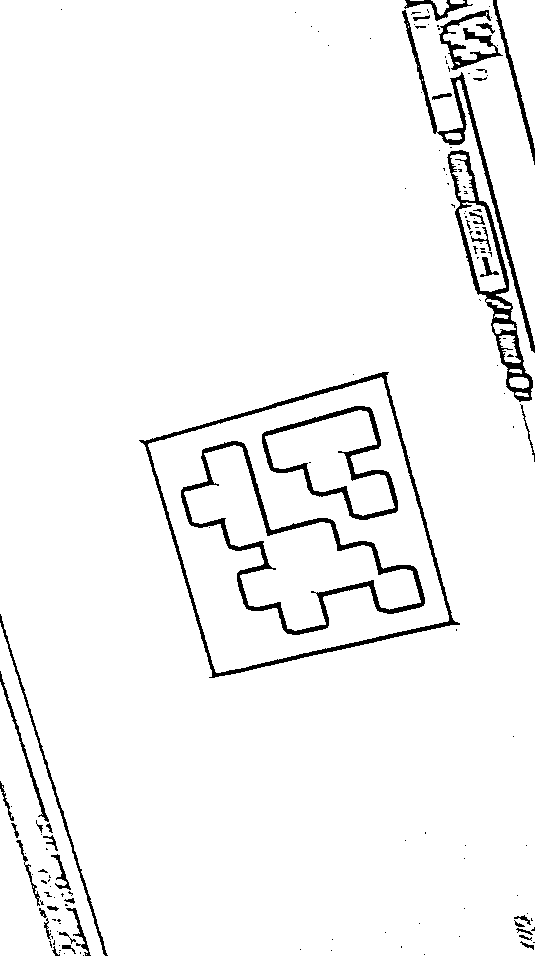
\includegraphics[scale=0.25]{img/threshold.png}
            \caption{Image seuillée}
        \end{figure}

        Une fois l'image binarisée, nous pouvons effectuer une détection de contours sur cette dernière.

        La méthode \verb|cv::findContours|, que nous utilisons fournie par OpenCV, renvoie pour chaque contour détecté une liste de points. Nous souhaitons à partir de ces points créer une forme qui va recouvrir le contour. Pour cela, nous allons générer une enveloppe convexe pour ces points.

        C'est à dire que nous allons englober de manière la plus optimale possible tous les points communs à un contour dans une forme convexe.

        \begin{figure}[!h]
            \centering
            
\includegraphics[scale=0.25]{img/convex_hull.png}
            \caption{Chaque contour de l'image est englobé}
        \end{figure}

        Certains contours détectés peuvent être formés de manière complexe (enchaînements de points pour au final un polygone avec un petit nombre de côtés) et risquerons de fausser la détection de contours quadrilatères. Pour chaque contours, nous effectuons un nettoyage. 

        Pour chaque triplet de points adjacents, les angles entre celui du milieu et les deux autres sont calculés. Si la différence est inférieur à un certain seuil (5\degree en pratique), le point du milieu est supprimé. Ainsi tous les points alignés sont supprimés. 

        Les coins peuvent contenir plusieurs points, non alignés, mais non nécessaire pour la détection. Nous créons alors des groupes de points adjacents avec une distance seuil (20 pixels en pratique). Puis chacun des groupes est remplacé un point, le centre du groupe.

        Avec ces contours désormais nettoyés, nous pouvons récupérer tous les contours d'exactement 4 sommets, qui correspondent à tous les candidats pour être le tag que nous recherchons.

        \subsection{Identification du tag correct}

        Tous les tags candidats sont ensuite comparés au modèle de tag que nous voulons reconnaître.

        \subsubsection{Homographie}
        \label{subsubsec:homographie}

        Le candidat sur l'image est déformé par rapport au modèle de tag qui sera nécessaire afin de comparer les deux images.

        Une première étape est en conséquence indispensable pour redresser cette image afin qu'elle soit de la même taille et forme que l'image à comparer.

        Nous allons pour ceci estimer l'homographie entre l'image avec le candidat déformé et un carré parfait, la forme qui est visée et qui correspond au modèle de tag que nous possédons.

        \begin{figure}[h]
            \centering
            \subfloat[][Tag candidat déformé]{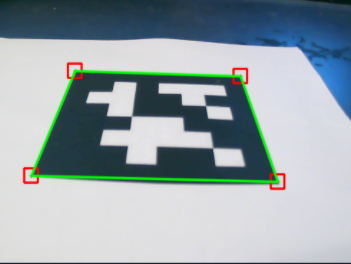
\includegraphics[width=0.48\linewidth]{img/beforewrap.png}}
            \hspace{.02\textwidth}
            \subfloat[][Forme visée]{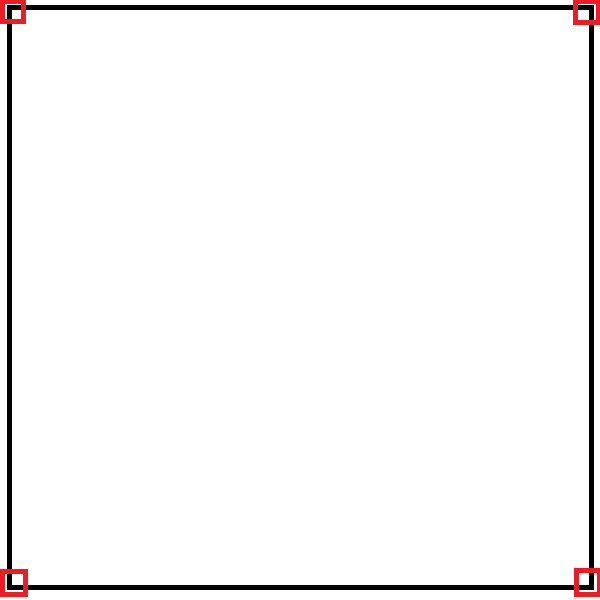
\includegraphics[width=0.38\linewidth]{img/tag_homography_target.png}}
            \caption{On cherche a estimer l'homographie entre ces deux représentations du tag candidat pour le redresser}
        \end{figure}

        L'estimation de l'homographie est en effet une transformation entre deux plans qui nous permettera de stocker dans une matrice d'homographie les informations relatives notamment à la rotation et translation entre ces deux plans.

        \textbf{\textit{Estimation de la matrice d'homographie}}

        Bien qu'OpenCV dispose de méthodes pour estimer une matrice d'homographie entre deux jeux de points, nous avons décidé de réimplémenter une solution afin de respecter le \emph{from scratch}.

        Comme vu précédemment, on cherche à établir la transformation entre deux images. C'est à dire, pour chaque couple de points $p_i \leftrightarrow p_{i}' $, nous cherchons la matrice $H$ telle que :
    
        \begin{center}
            $ p_i = Hp_i' $            
        \end{center}

        Avec :

        \begin{itemize}
            \item $ p_i $ correspondant aux points de départ, ou ici de l'image déformée.
            \item $ p'_i $ correspondant aux points d'arrivés, ou ici d'un cadre droit, la forme visée.
        \end{itemize}
            
        Nous pouvons développer donc pour tout point $p_i$ :
    
        \[
            \begin{pmatrix}
                x_i \\
                y_i \\
                1      
            \end{pmatrix}
            = 
            \begin{pmatrix}
                h1 & h2 & h3 \\
                h4 & h5 & h6 \\
                h7 & h8 & h9      
            \end{pmatrix} 
            \times
            \begin{pmatrix}
                x'_i \\
                y'_i \\
                1      
            \end{pmatrix}
            \]
        
        L'objectif est donc de déterminer la matrice H telle que :
    
        \begin{center}
        $ H = \begin{pmatrix} h1 & h2 & h3 \\ h4 & h5 & h6 \\ h7 & h8 & h9 \end{pmatrix} $
        \end{center}
    
        On peut réécrire l'estimation de l'homographie dans un premier temps pour un point de cette manière :

        \begin{center}
            $x_i = \frac{h1x'_i + h2y'_i + h3}{h7x'_i + h8y'_i + h9} $  
        \end{center}
    
        \begin{center}
            $y_i = \frac{h4x'_i + h5y'_i + h6}{h7x'_i + h8y'_i + h9} $
        \end{center}
    
        Qui est égal à :
    
        \begin{center}
            $ x'_ih1 + y'_ih2 + h3 - x'_i x_ih7 - y'_ix_ih8 - x_ih9 = 0 $
    
            $ x'_ih4 + y'_ih5 + h6 - x'_iy_ih7 - y'_iy_ih8 - y_ih9 = 0 $
        \end{center}

        Nous nous retrouvons sous la forme d'un système de 2 équations à 9 inconnues.

        On observe du coup qu'un couple de point mène donc à deux équations qui permettent de résoudre $H$.
    
        Nous pouvons d'ailleurs par avance résoudre h9, car dans le cas d'une homographie, nous avons toujours $h9 = 1$.
    
        Il nous reste huit inconnues à résoudre : 4 points sont alors nécessaires pour générer 8 équations dans le système, dont on considère $h9$ comme déjà résolu : 

        \[
        \begin{pmatrix} 
            x_1 & y_1 & 1 & 0 & 0 & 0 & -x_1 x'_1 & -y_1 x'_1 \\ 
            0 & 0 & 0 & x_1 & y_1 & 1 & -x_1 y'_1 & -y_1 y'_1 \\
    
            x_2 & y_2 & 1 & 0 & 0 & 0 & -x_2 x'_2 & -y_2 x'_2 \\ 
            0 & 0 & 0 & x_2 & y_2 & 1 & -x_2 y'_2 & -y_2 y'_2 \\
    
            x_3 & y_3 & 1 & 0 & 0 & 0 & -x_3 x'_3 & -y_3 x'_3 \\ 
            0 & 0 & 0 & x_3 & y_3 & 1 & -x_3 y'_3 & -y_3 y'_3 \\
    
            x_4 & y_4 & 1 & 0 & 0 & 0 & -x_4 x'_4 & -y_4 x'_4 \\ 
            0 & 0 & 0 & x_4 & y_4 & 1 & -x_4 y'_4 & -y_4 y'_4
        \end{pmatrix} 
        \times
        \begin{pmatrix} h1 \\ h2 \\ h3 \\ h4 \\ h5 \\h6 \\ h7 \\ h8 \end{pmatrix}
        =
        \begin{pmatrix} x'_1 \\ y'_1 \\ x'_2 \\ y'_2 \\ x'_3 \\ y'_3 \\ x'_4 \\ y'_4 \end{pmatrix} 
        \]
    
        Nous disposons de ces couples de points dans notre cas car nous avons déjà détecté d'une part les coins du tag candidat que l'on cherche à redresser, et d'autre part nous connaissons déjà les coordonnées des points d'arrivée, sous la forme d'un carré. Nous pouvons donc créer ce système d'équation à partir de ces quatre couples de points.

        Un pivot de Gauss est réalisé sur ce système d'équations. Une fois ce pivot résolu, nous obtenons une matrice en "row echelon form", c'est à dire :
    
        \begin{itemize}
            \item Toutes les lignes qui ne sont pas entièrement constituées de 0 commencent par un 1
            \item Pour deux lignes non constituées que de 0, la valeur 1 de la ligne placée en haut de la matrice sera plus à gauche que le 1 de la ligne placée plus bas
            \item Toutes les lignes avec seulement des 0 sont placées en bas
        \end{itemize}
    
        Nous effectuons en conséquence une "back substitution" pour faire apparaître la solution sur la dernière colonne.
    
        La dernière colonne du système est donc la résolution de la matrice $H$, qui nous donne notre matrice d'homographie.

        Cette méthode permet d'estimer de manière fiable la matrice d'homographie entre l'image avec le candidat et une image droite.

        
            \subsubsection{Wrap Perspective}

            Maintenant que la matrice d'homographie est établie, nous devons l'utiliser pour redresser l'image deformée dans la forme souhaitée.

            Pour chaque point de l'image d'arrivée, il faut appliquer la formule suivante :
            \begin{equation*}
                \text{dst}\left(x,y\right) = \text{src}\left(\frac{h1*x + h2*y + h3}{h7*x + h8*y + h9}, \frac{h4*x + h5*y + h6}{h7*x + h8*y + h9}\right)
            \end{equation*}
            avec $(x, y)$ le pixel courant. Étant donné que l'on cherche l'on cherche les pixels du carré, il faut d'abord inverser l'homographie.

            Cependant, dans le cas où la caméra aie prise l'image à l'envers, le tag candidat sera inversé par rapport au modèle à comparer. Le candidat, bien que valide, ne serait donc pas détecté. Pour contrer cela, nous allons par quatre fois effectuer une rotation sur l'ordre des points du contours pour tester toutes les orientations possibles. Cela permet également d'obtenir la bonne rotation lors de l'extraction de la matrice de projection (partie \ref{subsec:projection}).

        \begin{figure}[h]
            \centering
            \subfloat[][Image originale]{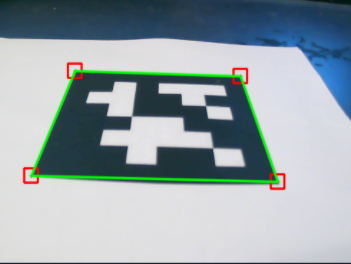
\includegraphics[width=0.48\linewidth]{img/beforewrap.png}}
            \hspace{.02\textwidth}
            \subfloat[][Tag potentiel extrait]{
\includegraphics[width=0.35\linewidth]{img/afterwrap.png}}
            \caption{Wrap Perspective sur la première image pour recadrer le tag potentiel}
        \end{figure}
            

        \subsection{Résumé de la procédure}

        Pour résumer, la détection du tag consiste à :

        \begin{itemize}
            \item Réaliser un seuillage adaptatif sur l'image
            \item Réaliser un convex hull sur les contours
            \item Nettoyer les contours
            \item Estimer l'homographie
            \item Effectuer la Wrap Perspective
            \item Comparer au modèle de tag
        \end{itemize}

    \subsection{Tracking}

    
    \section{Amélioration de la détection du tag}

    Après les premiers tests, nous avons remarqué que la détection du tag était efficiente lorsque le tag était bien visible quel que soit sa rotation ou sa taille, mais perdait en efficacité lors de mouvements plus brusques de la caméra, notamment à cause du flou de mouvement.

    Nous avons implémenté deux méthodes pour rendre plus robuste cette détection afin de détecter le tag même lors des mouvements de la caméra.

        \subsection{Défloutage gaussien}

        Une première méthode pour optimiser la détection du tag est de retirer le bruit causé par le flou de mouvement de la caméra lorsque le tag n'est pas détecté.

        Pour cela, on va considérer que le flou est causé par un flou gaussien. L'objectif est de soustraire l'image floutée par sa propre image non floutée.

        Nous appliquons un flou gaussien sur l'image bruitée. Ensuite, nous calculons la somme pondérée de l'image d'entrée et l'image floutée, avec un poids de $1.5$ pour l'image d'entrée et un poids de $-0.5$ pour l'image floutée. Nous prenons en réalité l'image bruitée par le flou de mouvement, auquel nous soustrayons l'image floutée par le filtre gaussien. Ceci permet d'éliminer une partie du flou sur l'image original et d'affiner les contours.

        \subsection{Marge d'acceptation de détection du tag}

        Comme nous l'avons vu précédemment, chaque tag potentiel détecté sur l'image est comparé au modèle de tag pour vérifier si les 64 cases du candidat correspondent bien au tag que nous cherchons.

        Lors du mouvement de la caméra, il peut arriver que le flou de mouvement empiète sur certaines cases et modifie légèrement le résultat, ce qui en conséquence écarte le tag de la recherche.

        Nous pouvons en conséquence tolérer un seuil d'acceptation du tag, où si jamais entre 5 et 10 \% des cases du potentiel tag ne corrèlent pas au modèle, le candidat est quand même accepté comme étant le tag, car si observons une correspondance par exemple sur 56 cases du tag sur les 64, nous pouvons être quasiment sûr qu'il s'agit bien du tag que nous recherchons.

        \subsection{Résultats}

        Les deux méthodes indépendamment améliorent, mais pas de façon considérable, les résultats, mais en les combinant nous parvenons à avoir une détection plus robuste.

        \begin{figure}[!h]
            \begin{center}
                \begin{tabular}{ | c | c | c | c | c | }
                \hline
                Vidéo & Sans optimisation & Approximation & Défloutage Gaussien & Combinaison \\ \hline
                Vidéo 1 & 88.2\% & 91.4\% & 90.9\% & 94.1\% \\ \hline
                Vidéo 2 & 12.21\% & Non testé & Non testé & 37.40\% \\
                \hline
                \end{tabular}
        \end{center}
        \caption{Taux de détection du tag par vidéo}
        \end{figure}

        Vidéo 1 : Vidéo de plutôt bonne qualité, le tag sort de l'écran une seconde

        Vidéo 2 : Vidéo de mauvaise qualité, plus de mouvement de la caméra, le tag est plus petit et légèrement froissé.

        Bien que la détection avec ces méthodes reste généralement de bonne qualité, il y a malgré tout plus de risque d'avoir une détection d'être dégradée, comme il peut être observé sur l'image ci-dessous.

        \begin{figure}[!h]
            \centering
            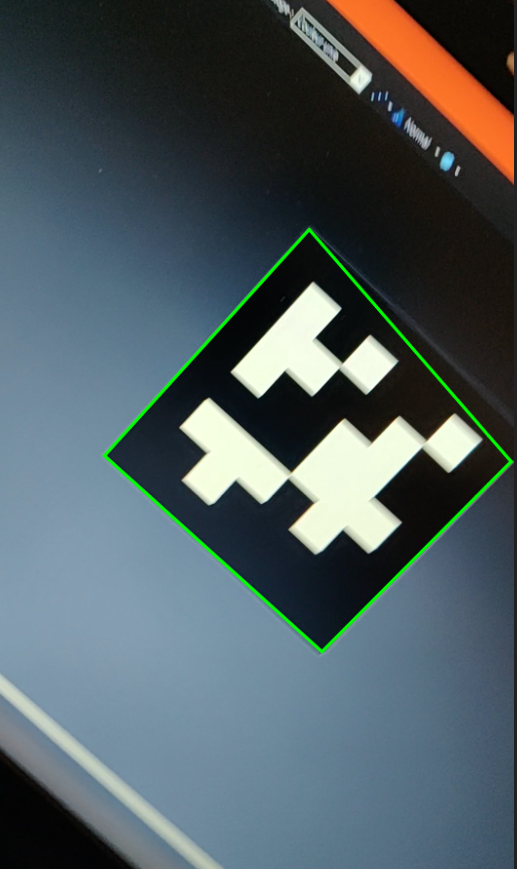
\includegraphics[scale=0.25]{img/cropped_tag.png}
            \caption{Le tag est détecté, mais un angle n'est pas bien géré}
        \end{figure}

        Pour éviter de dégrader la détection des contours lors des frames suivantes du flux vidéo, nous ne réalisons pas de tracking sur le tag que nous avons détecté à l'aide des méthodes d'optimisations, car il sera éventuellement possible de trouver un tag parfait lors de la frame suivante, qui serait de meilleur qualité qu'un tag de moins bonne qualité tracké par rapport à celui de la frame précédente.

        Cette petite marge d'erreur permet entre autre également de gérer partiellement l'occlusion du tag. En effet, un obstacle de petite taille cachant seulement quelques cases du tag peut ne pas poser de problème à sa détection, étant donné que les autres cases du tag seraient tout de même détectées.

        IMAGE OCCULSION TAG ? 

        De plus, ces méthodes d'optimisations ne permettent pas de détecter le tag lorsqu'il sort de l'écran.
    \part{Rendu}
    Après avoir détecter le tag dans l'image, la seconde grande étape est de projeter un modèle 3D sur la scène. Pour cela, l'utilisateur indique au lancement du programme le ou les modèles à utiliser, avec ou non des matériaux, et ceux-ci seront rendus à chaque image.

    \section{Gestion des objets}

        \subsection{Objets}

            \subsubsection{Définition du format}                
                Un objet 3D est composé de sommets, formant des faces d'au moins 3 côtés. Le format le plus simple pour stocker un modèle 3D est le \emph{.obj}. Cette norme définie les sommets, les matériaux et les normales pour chaque face dans un format texte. Chaque ligne débute par un indicateur puis les valeurs à proprement parler. Un exemple est visible figure \ref{fig:obj}. Nous utilisons 4 indicateurs :
                \begin{itemize}
                    \item v x y z : sommet à la position $(x, y, z)$
                    \item vt u v [w] : coordonnées de texture (voir partie \ref{subsubsec:materiaux})
                    \item vn x y z : normale (voir partie \ref{subsubsec:lumiere})
                    \item f v/vt/vn [...] : les faces de l'objet avec un triplet d'indice pour chaque sommet (minimum 3). La coordonnée de texture peut être vide (v//vn).
                \end{itemize}
                
                \begin{figure}[h]
                    \centering
                    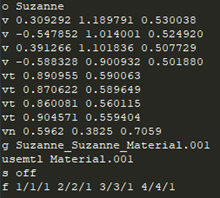
\includegraphics[scale=0.8]{img/rendu/obj.png}
                    \caption{Exemple de fichier \emph{.obj}}
                    \label{fig:obj}
                \end{figure}
                Nous avons écrit un parser afin de décomposer ce fichier \emph{.obj}.

                Chaque objet est contenu dans une classe \emph{Object}. Celle-ci contient un ensemble de face qui correspond à plusieurs points, une couleur et une normale. Plusieurs fonctions sont également disponible afin de manipuler l'objet : \emph{rotate}, \emph{scale}, \emph{position}\dots

            \subsubsection{Matériaux}
            \label{subsubsec:materiaux}

            Afin de rendre les objets plus agréables à l'\oe il, nous avons décider d'implémenter la gestion des matériaux. Nous utilisions déjà le format \emph{.obj} pour les modèles, il semblait donc naturel d'utiliser les \emph{.mtl}, format défini par la même norme, pour les matériaux. 

            Un fichier \emph{.mtl} est un fichier texte, et nous utilisons uniquement une seule ligne de ce fichier, \emph{map\_kD}, qui indique le nom de l'image texture utilisée. Les coordonnées de texture renseignées dans le \emph{.obj} indiquent des pourcentage dans cette image, respectivement $u$, $v$, la largeur et la hauteur. Nous travaillons ici avec des images 2D.

            \begin{figure}[h]
                \centering
                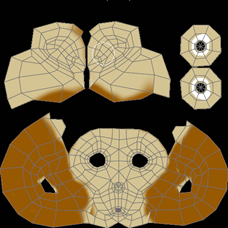
\includegraphics[scale=0.8]{img/rendu/texture.png}
                \caption{Texture découpée par face}
                \label{fig:texture}
            \end{figure}

            Dans la figure \ref{fig:texture}, nous pouvons voir les faces en fonction des coordonnées indiquées pour chaque sommet. Afin de pouvoir utiliser cette texture, il faut déformer le polygone (en utilisant une homographie) pour l'appliquer sur le polygone projeté. Cependant, cette étape est très coûteuse en performance car il faut l'appliquer à chaque polygone de chaque objet à chaque image de la vidéo. Nous avons alors choisi de préférer le temps réel et, pour cela, une face ne possède qu'une seule couleur, inscrite directement dans la classe \emph{Object}. Pour choisir la couleur, nous prenons simplement la couleur du pixel au centre du polygone sur l'image texture. Cela nous donne alors un objet avec des couleurs unies pour les faces. 
            
            Une amélioration possible du programme pourrait être de prendre en compte les autres paramètres du fichier \emph{.mtl} et donc de ne pas obligatoirement utiliser d'image pour la texture.

        \subsection{Scène}

            La scène est un regroupement de tous les objets et de la caméra. Afin de donner une liberté à l'utilisateur et de ne pas recompiler à chaque fois le programme, nous avons défini un format CSV \emph{.scene} (figure \ref{fig:scene}) qui défini chaque objet de la scène ainsi que leur position et leur rotation.

            \begin{figure}[h]
                \centering
                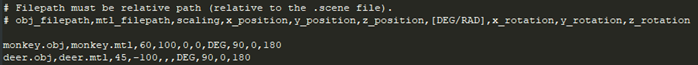
\includegraphics[scale=0.8]{img/rendu/scene.png}
                \caption{Fichier CSV \emph{.scene}}
                \label{fig:scene}
            \end{figure}

            Chaque champ est optionnel, à l'exception du premier qui défini l'objet à charger. Un champ vide prendra une valeur par défaut inscrite dans le code.

            Notre méthode pour le placement et l'échelle des objets à cependant un défaut. Il faut déterminer à la main la bonne position et la bonne échelle pour que l'objet soit visible et au bon endroit. En effet, deux logiciels de modélisation n'enregistre pas l'échelle de la même façon. Par exemple, avec Blender, une échelle entre 45 et 55 est idéale. Tous les \emph{.obj} fournis dans le projet ont été créés par nous-même sous Blender.

        \subsection{Lumière}
        \label{subsubsec:lumiere}

        Une méthode d'ombrage plat (\textit{Flat Shading}) a été implémentée afin de rendre l'apparence des objets plus réaliste. La lumière est représentée par un vecteur qui donne sa direction. Afin de déterminer l'éclairage d'une face, nous utilisons la normale définie dans le \emph{.obj}. Nous ne souhaitons qu'une seule illumination par face, nous calculons alors la moyenne des normales des sommets que nous enregistrons dans la face avec la couleur et les points. 

        Ensuite, la luminosité est calculée pour chaque face en fonction de l'angle entre sa normale et la direction de la lumière. Plus l'angle est proche de 0\degree, plus les vecteurs sont alignés et donc plus la face est dans l'ombre. Inversement, plus l'angle est proche de 180\degree, plus la face est éclairée. Cet angle est normalisé puis multiplié à la couleur de la face. Nous pouvons voir cette effet, avec les matériaux, dans la figure \ref{fig:lumiere}. Le rendu sera expliqué dans la partie suivante.

        \begin{figure}[h]
            \centering

            \subfloat[][]{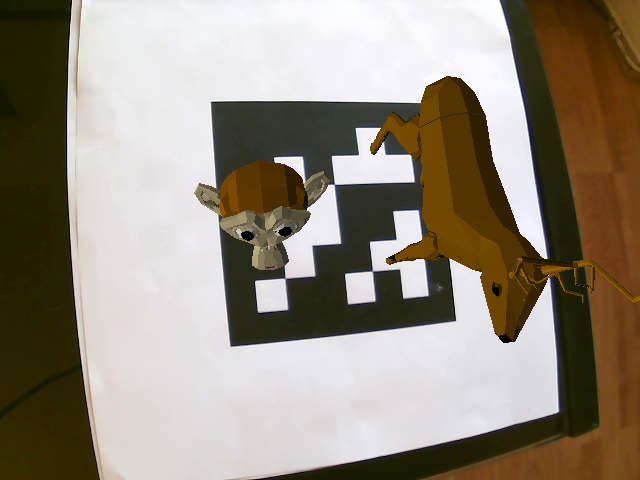
\includegraphics[width=0.49\linewidth]{img/rendu/flat_shading_left.png}}
            \hspace{.005\textwidth}
            \subfloat[][]{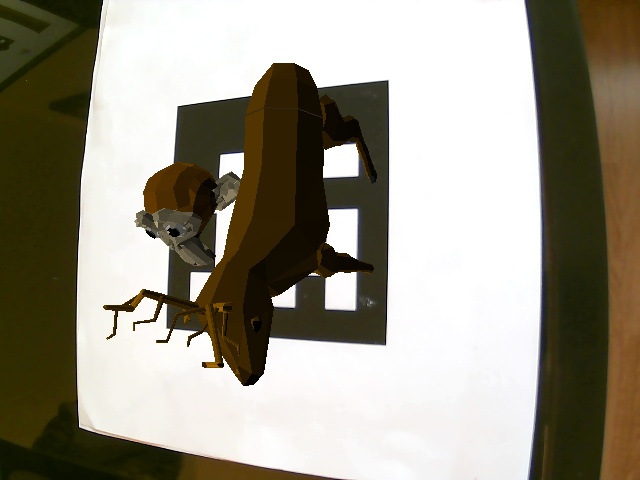
\includegraphics[width=0.49\linewidth]{img/rendu/flat_shading_right.png}}

            \caption{Ombrage plat sur les objets à partir d'une source lumineuse venant de la gauche}
            \label{fig:lumiere}
        \end{figure}

    \section{Caméra et projection}
        Après avoir chargé les objets dans la scène 3D, il faut les projeter sur l'image en fonction du tag. Nous utilisons cette relation :
        \begin{equation*}
            \begin{pmatrix}
                u \\ v \\ 1
            \end{pmatrix}
            = K.E.
            \begin{pmatrix}
                x_w \\ y_w \\ z_w \\ 1
            \end{pmatrix}
        \end{equation*}
        avec $u,v$ les coordonnées dans le plan image en pixels, $K$ les paramètres intrinsèques de la caméra, $E$ les rotations et translation de la caméra dans le repère monde et $x_w, y_w, z_w$ les coordonnées du point 3D dans le repère monde.

        \subsection{Calibration}
            Afin de déterminer les paramètres intrinsèques de la caméra, nous avons développé une fonction pour les calculer. Elle se base sur la prise de photos de checkerboard tel que la figure \ref{fig:checkerboard}.

            \begin{figure}[!h]
                \centering
                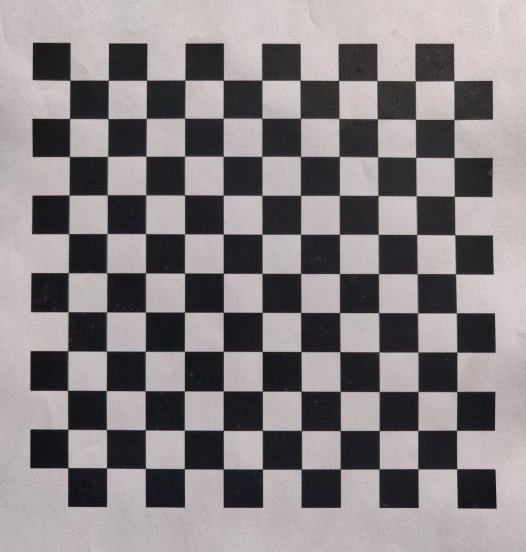
\includegraphics[scale=0.3]{img/rendu/checkerboard.jpg}
                \caption{Exemple de checkerboard}
                \label{fig:checkerboard}
            \end{figure}

            Des images de différents angles sont nécessaires. Après quelques essais, environ 5-6 images sont suffisantes pour estimer les paramètres. La méthode se base principalement sur la fonction \verb|cv::calibrateCamera| d'OpenCV. Elle prend en paramètres les coordonnées des points 3D et leur correspondance sur l'image (les points 2D). Étant donné que le checkerboard est connu, on peut donner des coordonnées à chaque coins des carrés en supposant que $z=0$, ces points étant sur le même plan. Les coins du checkerboard sur l'image peuvent être trouvés par la fonction \verb|cv::findChessboardCorners| d'OpenCV.

            Après avoir calculer les paramètres intrinsèques, nous les enregistrons dans un format texte avec l'extension \emph{.cam} (figure \ref{fig:cam})

            \begin{figure}[!h]
                \centering
                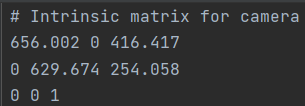
\includegraphics[scale=0.8]{img/rendu/cam.png}
                \caption{Fichier \emph{.cam} représentant les paramètres intrinsèques}
                \label{fig:cam}
            \end{figure}

            Ce fichier se compose d'une matrice 3x3 représentant les paramètres intrinsèques ainsi :
            \begin{equation*}
                \begin{pmatrix}
                    f_x & s & x_0 \\
                    0 & f_y & y_0 \\
                    0 & 0 & 1
                \end{pmatrix}
            \end{equation*}
            $f$ est la distance focale en pixels. Dans une caméra parfaite, $f_x$ et $f_y$ sont égaux mais en pratique, ils peuvent différer, ce qui cause des pixels non carrés. $s$ est une distortion de l'image, souvent égale à 0, ce qui est suffisant dans notre cas. Enfin $(x_0, y_0)$ est le centre optique de l'image, l'intersection entre l'axe optique et le plan image. Il est en général plus ou moins au centre de l'image. 

        \subsection{Projection}
        \label{subsec:projection}
            Ayant les paramètres intrinsèques de la caméra, nous pouvons maintenant rendre les objets 3D. À chaque frame, nous devons mettre à jour la matrice de projection de la caméra.

            \subsubsection{Matrice de projection}
                La matrice de projection est la multiplication matricielle de $K$ et $E$. Après l'avoir calculé, il suffit donc de la multiplier à un point 3D pour avoir ses coordonnées dans le plan image.

                Afin de mettre à jour la matrice de projection, nous calculons tout d'abord une homographie $H_i$ entre les points du tag et un carré parfait comme défini dans la partie \ref{subsubsec:homographie}. Le calcul de l'homographie est une opération inversible, on peut facilement calculer l'homographie allant du carré parfait aux points du tag en inversant la matrice $H_i$, ce qui nous donne une matrice $H$. L'homographie $H$ contient les mêmes informations que la position la caméra $K.E$ ($E = [R|t]$). Il est nécessaire de la normaliser. 

                On peut donc estimer la position de la caméra ainsi :
                $R^1$ et $R^2$ sont les premières colonnes de $H$. $t$ est la dernière colonne de $H$. Étant donné que les rotations doivent être orthogonales, car on se place dans un repère orthonormé 3D, on peut calculer $R^3$ avec le produit vectoriel de $R^1$ et $R^2$ donc $R^3 = R^1 \times R^2$.

                En résumé nous avons :
                \begin{equation*}
                    E = [R|t] = [H^1 | H^2 | H^1\times H^2 | H^3]
                \end{equation*}
                Nous pouvons donc calculer $K.E$, la matrice de projection.
                
                Chaque point d'une face est alors projeté sur l'image en multipliant $K.E$ par le point. On utilise des coordonnées homogènes, il est donc nécessaire de diviser $u$ et $v$ par la troisième coordonnée afin d'obtenir 1 à cette dernière. 

                Le polygone projeté est alors rempli en utilisant la fonction \verb|cv::fillConvexPoly| avec la couleur de la face multiplié par sa luminosité (voir partie \ref{subsubsec:lumiere}). Nous pouvons voir le résultat de ces opérations dans la figure \ref{fig:sans_peintre}.

                \begin{figure}[!h]
                    \centering
                    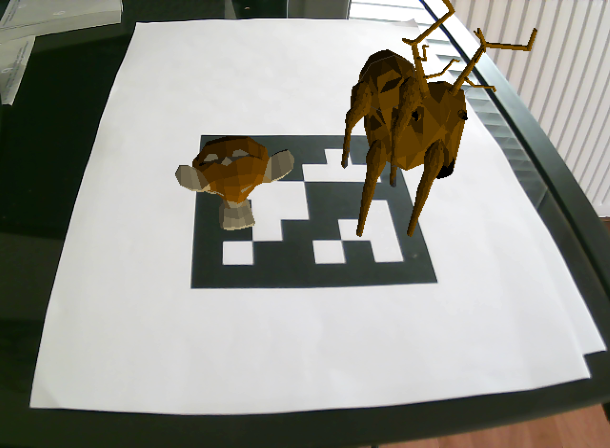
\includegraphics[scale=0.45]{img/rendu/sans_peintre.png}
                    \caption{Rendu d'une scène sans l'algorithme du peintre}
                    \label{fig:sans_peintre}
                \end{figure}
                
            \subsubsection{Algorithme du peintre}
                Nous pouvons tout de suite voir un problème dans la figure \ref{fig:sans_peintre}, les faces arrières sont parfois dessinées sur les faces avant, ce qui rend l'image très confuse. Le moyen le plus simple de le résoudre est l'algorithme du peintre. Il consiste à dessiner les faces les plus loins en premier puis se rapprocher de la caméra petit à petit. Ainsi les polygones les plus proches vont recouvrir les autres. 

                \begin{figure}[!h]
                    \centering
                    
\includegraphics[scale=0.3]{img/rendu/peintre_probleme.png}
                    \caption{Agencement de polygones problématique}
                    \label{fig:peintre_probleme}
                \end{figure}

                Cet algorithme n'est pas parfait et peut ne pas fonctionner dans certains cas d'utilisation précis, comme celui de la figure \ref{fig:peintre_probleme}. Il n'est non plus très efficient car il demande de calculer des faces qui seront cachés par la suite. Cependant, il est suffisant à notre cas et a donc été choisi. 

                Nous extrayons tout d'abord la translation de la caméra de la matrice de projection suivant cette formule : 
                \begin{equation*}
                    E = K^{-1}.K.E = [R|t]
                \end{equation*}
                Grâce à cela, nous pouvons calculer la distance à la caméra d'une face en prenant la norme de la différence du vecteur $t$ et du centre de la face. En utilisant ce calcul, il est possible de trier les faces en fonction de leur distance. Il suffit simplement par la suite de projeter par les faces les plus loins en premier. Nous obtenons donc ainsi un rendu réaliste visible à la figure \ref{fig:avec_peintre}.

                \begin{figure}[!h]
                    \centering
                    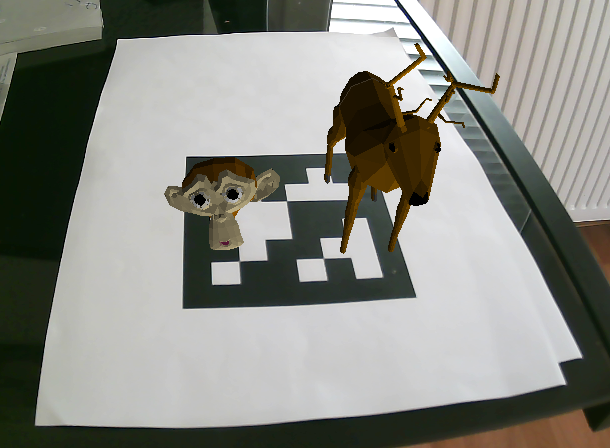
\includegraphics[scale=0.45]{img/rendu/avec_peintre.png}
                    \caption{Rendu d'une scène avec l'algorithme du peintre}
                    \label{fig:avec_peintre}
                \end{figure}

                Les différents objets sont gérés simplement en regroupement toutes les faces de tous les objets avant de les trier pour les projeter. 


    \newpage
\addpart{Perspectives d'améliorations}

\section{Détection de tag}

    \subsection{Robustesse de la détection}

    Une des faiblesses de notre système de détection de tag est l'impossibilité du système à détecter le tag lorsque ce dernier n'est pas entièrement dans l'écran.

    Implémenter une méthode permettant justement de réussir à estimer la position du tag à partir d'un fragment visible de ce dernier aurait pu s'avérer intéressant, les mouvements de l'utilisateur pouvant faire sortir régulièrement le tag du champ de la caméra.

\section{Techniques de rendu}

    \subsection{Performance}

    \subsection{Détection des sources lumineuses}

    La lumière dans ce système de réalité augmenté est géré statiquement : le vecteur représentant la direction de la lumière est invariant selon l'image.

    Détecter les sources lumineuses sur l'image pour modifier image par image la direction de la lumière aurait pu être une manière intéressante d'augmenter le réalisme de l'application, bien que cette détection de source de lumière sur l'image se serait avéré être une tâche probablement nécessitant du temps.

    \subsection{Ombrage de Gouaraud}

    Nous avons tenté d'implémenter, sans succès, un ombrage de Gouraud pour le rendu des objets. Cela aurait pu s'avérer intéressant pour un souci de réalisme, l'ombrage de Gouraud interpolant chaque pixel de chaque face pour lui assigner une luminosité différente.

    Malheureusement, OpenCV n'est pas l'outil le plus adapté à ce genre de tâche et les calculs étaient particulièrement long à être effecutés. Pour parvenir plus facilement à un résultat, nous aurions pu utiliser un moteur de rendu ou paralléliser le calcul.

    \begin{figure}[!h]
        \centering
        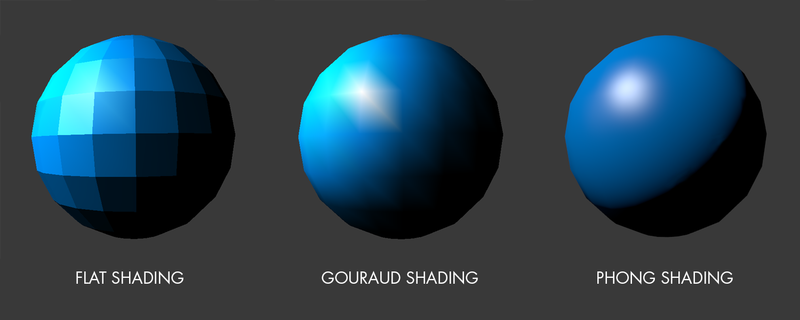
\includegraphics[scale=0.25]{img/shading.png}
        \caption{L'interpolation utilisée dans l'ombrage de Gouraud et de Phong lisse la surface de l'objet et améliore le réalisme du rendu}
    \end{figure}
    \part{Implémentation}

Le projet est découpé en différentes classes. La description de chaque classe est disponible dans le dossier \emph{documentation/}. Ce projet défini un namespace \emph{arfs} où toutes les fonctionnalités sont contenues. Il existe également plusieurs sous-namespaces :
\emph{
\begin{itemize}
    \item arfs::Utils
    \item arfs::Utils::Geometry
    \item arfs::Utils::Image
    \item arfs::Utils::CV
    \item arfs::Renderer
\end{itemize}
}
\section*{Arguments en ligne de commande}
Afin de rendre l'utilisation plus simple, nous avons ajouté un certain nombre d'arguments pour lancer le programme en ligne de commande avec différents paramètres. Le tableau \ref{table:args} précise chacun des arguments disponibles.

\begin{table}[h]
    \centering
    \begin{tabularx}{\textwidth}{|l|X|}
        \hline
        Argument & Description \\ \hline \hline
        \verb([--webcam | -w] id( & Utilise une webcam comme entrée video. L'id est un nombre et commence à 0 pour la première webcam branchée.  \\ \hline
        \verb([--video | -v] filename( & Utilise une vidéo comme entrée video \\ \hline
        \verb([--tag | -t] filename( & Chemin de l'image du tag à détecter \\ \hline
        \verb([--camera-parameters | -p] filename( & Chemin du fichier \emph{.cam} contenant les paramètres intrinsèques de la caméra \\ \hline
        \verb([--scene | -s] filename( & Chemin du fichier \emph{.scene} \\ \hline
        \verb([--calibrate | -c]( & Flag pour calibrer ou non la caméra\\ \hline
        \verb(--checker-size-width size( & Taille en largeur du checkerboard\\ \hline
        \verb(--checker-size-height size( & Taille en hauteur du checkerboard\\ \hline
        \verb(--images-folder( & Chemin du dossier contenant les images (ou où sauvegarder les images) de calibration \\ \hline
        \verb([--take-pictures]( & Flag permettant de prendre des images pour la calibration \\ \hline
        \verb([--help | -h]( & Affiche l'aide \\
        \hline
    \end{tabularx}
    \caption{Arguments en ligne de commande}
    \label{table:args}
\end{table}

    \rhead{\bsc{Conclusion}}

    \part*{Conclusion}
\addcontentsline{toc}{part}{Conclusion}

Ce projet a été extrêmement formateur. Nous avons pu implémenter nombre de concepts vus dans les cours d'IN5x et ainsi mieux les comprendre. Les problèmes que nous avons rencontrés lors de l'implémentation nous ont permis de saisir les petits détails.

Cette application de réalité augmentée est loin d'être parfaite et, comme expliqué dans la partie \hyperref[part:ameliorations]{Amélioration}, nombre de perfectionnement reste à réaliser. Nous aurions pu obtenir un meilleur rendu et plus rapidement si nous avions utilisé les outils déjà disponibles, par exemple le module \verb|ArUco| d'OpenCV pour la détection du tag et un moteur de rendu tel qu'OpenGL, mais nous pensons que les connaissances que nous avons acquises justifient largement ce choix. 
    

\end{document}